% This is samplepaper.tex, a sample chapter demonstrating the
% LLNCS macro package for Springer Computer Science proceedings;
% Version 2.20 of 2017/10/04
%
\documentclass[runningheads]{llncs}
%
\usepackage{graphicx}
\usepackage{tikz}
\usepackage{subcaption}
\captionsetup{compatibility=false}
\usetikzlibrary{matrix}
% Used for displaying a sample figure. If possible, figure files should
% be included in EPS format.
%
% If you use the hyperref package, please uncomment the following line
% to display URLs in blue roman font according to Springer's eBook style:
% \renewcommand\UrlFont{\color{blue}\rmfamily}

\begin{document}
%
\title{COMP 6721: Double Card}
\author{Martin Khannouz}
%
\institute{40093517 \email{martin.khannouz@gmail.com}}
%
\maketitle              % typeset the header of the contribution
%
\section*{Introduction}
This project report describes how the first
project of \textit{Introduction to Artificial
Intelligence} was developed. The first section
covers the environment and the tools used for the
project. The heuristic section describes each
%TODO Briefly describe what a heuristic is.
heuristic and how they were improved. The
difficulties section summarizes the difficulties
encountered during the project and how they were
overcome.

\section{Settings and Structures}
\subsection{Settings}
The developing part of this project was realized
on an Archlinux distribution with Python~3.7.2.
Vim with the Jedi plugin was used to code and a private Github repository was set to
keep track of the changes.
The \textit{orwell} machine was used before each
deliverable to ensure the project worked with the
software version on Concordia's computers. Pytest
was used to guarantee no regression has been made.

\subsection{Stucture}
The project is structured in classes with
the main one representing the engine. This class is an
instance of the game and implements the rules.
To ensure this class operates properly, unit tests
were implemented before the class methods, based on
the use cases given by the teacher.
This class was optimized as much as possible to
guarantee the fastest execution time for
\textit{MinMax} algorithm.

The project also contains three types of players. A
\textit{Human} player that parse the input from the command
line. A \textit{MinMax} player that implement tweaked
minimax version with alpha-beta pruning. The
\textit{MonteCarlo} player which was supposed to implement
a Monte Carlo Tree Search even though it was a
complete failure due to my poor understanding of
this algorithm. Finally, a random player was
developed during the early stage of the project.
This "algorithm" served as a control test for other
player types because none of them should lose
against such a chaotic player\footnote{Based on my
statistics, even a 5-years old kid should get a
win rate of 50\%.}.

Automatic players (\textit{MinMax} and
\textit{MonteCarlo}) rely on heuristic to complete
their search. All heuristic functions are grouped
in one file: \textit{heuristic.py}.
Finally, the class \textit{Move} represents a move
that could be played.

In addition to these classes, additional functions
were implemented. One function used genetic
algorithms to optimize the \textit{Vspace}
heuristic, but it was too slow and just gave a hint
of how to enhance the heuristic rather than
accurate weights.  A win rate function was also
implemented to compare combinations of player and
heuristic against each other. Finally, a
non-tweaked MinMax version was developed for
deliverable 2.

\subsection{Tweaks in \textit{MinMax}}
The original \textit{MinMax} algorithm explores the
complete tree of possibilities and applies the
heuristic function on the leaf. However, the
heuristic functions described below do not take
into account who won first. For instance, a sequence of
move could be preferred if a player scores three
lines of four symbols even if his opponent already won at
the previous move.

To prevent this behavior, the MinMax algorithm was
tweaked to check for winning condition after
playing each possible move at any depth. This
modification prevents the exploration of game
states already won by a player.

Even though calling the winning function from the
engine was costly at the beginning of the project,
I managed to drastically reduce this time by
improving the performances.

To prevent exceeding the six-second limit, a timer
was added in the MinMax algorithm. If this limit
was reached, the algorithm stops and returns the
best move encountered until this time.

The \textit{MinMax} algorithm contains a parameter
to sort the moves at each level. This approach was
supposed to prune the state space faster. At the
beginning of the project, this sort improved
significantly the performance, but on later
versions of the heuristics, it slowed the algorithm.
Therefore, it was barely used nor study.

Finally, when the algorithm runs on an empty
board, it returns a random vertical move. A
vertical move because the heuristics appear to
have a better winning rate when they start with
this move type. The move was randomly picked to
explore openings and to bring small changes from one game to another.
\section{Heuristics}
%TODO add citation to wikipedia for heuristics
%TODO add importance of the heuristic in minmax
Five heuristics were developed in this project
even though only two were made for competitive
use. One heuristic is the naive function for the
second deliverable. Another is a random heuristic
that systematically returns a new random number. It
was used to spot runtime errors in \textit{MinMax} and
\textit{MonteCarlo} algorithms. The \textit{Basic}
heuristics only check for winning situations and
was used for basic controls.
The two other heuristics are described in
subsections of their own.

\subsection{Convolution}
The convolution utilizes the \textit{convolve2d} function
from Scipy to estimate the value of a current
state.
The game board is split into two matrices: dot and
color. Each matrix contains -1, 0, or 1. A zero
indicates an empty space while the two other values
represent either a filled dot and an empty dot, or
a white cell and a red cell.
Applying \textit{convolve2d} on these matrices
produces new matrices with values that range from
-4 to 4. A cell with an absolute value of four indicates a row
of four and therefore, a winning position.
The heuristic gathers all intermediate values into
a histogram (using the \textit{histogram}
function of numpy) then give a weight to each
value. For instance, a weight of 16 was given to
each intermediate value of 3 which represent a row
of three.

Figure~\ref{fig:board-example} shows an example of
the board. Figure~\ref{fig:dot-representation}
focuses on the dot player and show the
transformation applied to the board for this
player. Filled dots are set to 1 and circles to
-1. Zeros are not represented for more clarity.
The heuristic applies four convolutions: one for
the rows, another for the columns and one for each
diagonal. These convolutions generate four smaller
matrices showed in
Figure~\ref{fig:convolution-results} (left side).
The matrices are then flattened, concatenated and the
absolute value is applied to every cell. Finally,
the histogram is built out of this matrix and each
element is multiplied by a weight before being
summed.  The final
value of the board is the difference between the
two player values.

This approach is strong for many reasons. It is
faster than calling python code because Scipy and
Numpy rely on C written functions. Incomplete rows
that contain zeros are more valued than incomplete
rows that contain opposite values. Finally,
because the convolution mask is applied to empty
spaces, the heuristic can build complex
structures with space in the middle or above.

\begin{figure}[ht]
		\center
		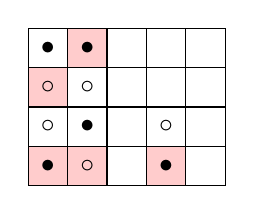
\begin{tikzpicture}

				\node [draw, fill=red!20, minimum width=0.5cm, minimum height=0.5cm] at (0, 0) {$\bullet$};
				\node [draw, fill=red!20, minimum width=0.5cm, minimum height=0.5cm] at (0.5, 0) {$\circ$};
				\node [draw, minimum width=0.5cm, minimum height=0.5cm] at (1.0, 0) {};
				\node [draw, fill=red!20, minimum width=0.5cm, minimum height=0.5cm] at (1.5, 0) {$\bullet$};
				\node [draw, minimum width=0.5cm, minimum height=0.5cm] at (2.0, 0) {};


				\node [draw, minimum width=0.5cm, minimum height=0.5cm] at (0, 0.5) {$\circ$};
				\node [draw, minimum width=0.5cm, minimum height=0.5cm] at (0.5, 0.5) {$\bullet$};
				\node [draw, minimum width=0.5cm, minimum height=0.5cm] at (1.0, 0.5) {};
				\node [draw, minimum width=0.5cm, minimum height=0.5cm] at (1.5, 0.5) {$\circ$};
				\node [draw, minimum width=0.5cm, minimum height=0.5cm] at (2.0, 0.5) {};


				\node [draw, fill=red!20, minimum width=0.5cm, minimum height=0.5cm] at (0, 1) {$\circ$};
				\node [draw, minimum width=0.5cm, minimum height=0.5cm] at (0.5, 1) {$\circ$};
				\node [draw, minimum width=0.5cm, minimum height=0.5cm] at (1.0, 1) {};
				\node [draw, minimum width=0.5cm, minimum height=0.5cm] at (1.5, 1) {};
				\node [draw, minimum width=0.5cm, minimum height=0.5cm] at (2.0, 1) {};

				\node [draw, minimum width=0.5cm, minimum height=0.5cm] at (0, 1.5) {$\bullet$};
				\node [draw, fill=red!20, minimum width=0.5cm, minimum height=0.5cm] at (0.5, 1.5) {$\bullet$};
				\node [draw, minimum width=0.5cm, minimum height=0.5cm] at (1.0, 1.5) {};
				\node [draw, minimum width=0.5cm, minimum height=0.5cm] at (1.5, 1.5) {};
				\node [draw, minimum width=0.5cm, minimum height=0.5cm] at (2.0, 1.5) {};

		\end{tikzpicture}
		\caption{An example of a board game. Cards are not represented.}
		\label{fig:board-example}
\end{figure}
\begin{figure}[ht]
		\center
		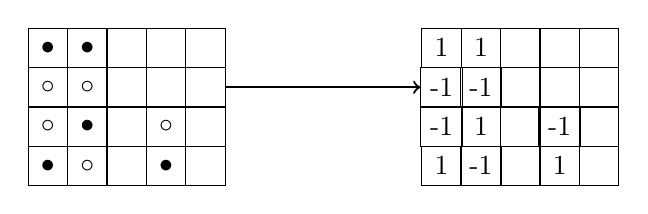
\begin{tikzpicture}

				\node [draw, minimum width=0.5cm, minimum height=0.5cm] at (0, 0) {$\bullet$};
				\node [draw, minimum width=0.5cm, minimum height=0.5cm] at (0.5, 0) {$\circ$};
				\node [draw, minimum width=0.5cm, minimum height=0.5cm] at (1.0, 0) {};
				\node [draw, minimum width=0.5cm, minimum height=0.5cm] at (1.5, 0) {$\bullet$};
				\node [draw, minimum width=0.5cm, minimum height=0.5cm] at (2.0, 0) {};


				\node [draw, minimum width=0.5cm, minimum height=0.5cm] at (0, 0.5) {$\circ$};
				\node [draw, minimum width=0.5cm, minimum height=0.5cm] at (0.5, 0.5) {$\bullet$};
				\node [draw, minimum width=0.5cm, minimum height=0.5cm] at (1.0, 0.5) {};
				\node [draw, minimum width=0.5cm, minimum height=0.5cm] at (1.5, 0.5) {$\circ$};
				\node [draw, minimum width=0.5cm, minimum height=0.5cm] at (2.0, 0.5) {};


				\node [draw, minimum width=0.5cm, minimum height=0.5cm] at (0, 1) {$\circ$};
				\node [draw, minimum width=0.5cm, minimum height=0.5cm] at (0.5, 1) {$\circ$};
				\node [draw, minimum width=0.5cm, minimum height=0.5cm] at (1.0, 1) {};
				\node [draw, minimum width=0.5cm, minimum height=0.5cm] at (1.5, 1) {};
				\node [draw, minimum width=0.5cm, minimum height=0.5cm] (A) at (2.0, 1) {};

				\node [draw, minimum width=0.5cm, minimum height=0.5cm] at (0, 1.5) {$\bullet$};
				\node [draw, minimum width=0.5cm, minimum height=0.5cm] at (0.5, 1.5) {$\bullet$};
				\node [draw, minimum width=0.5cm, minimum height=0.5cm] at (1.0, 1.5) {};
				\node [draw, minimum width=0.5cm, minimum height=0.5cm] at (1.5, 1.5) {};
				\node [draw, minimum width=0.5cm, minimum height=0.5cm] at (2.0, 1.5) {};

				\node [draw, minimum width=0.5cm, minimum height=0.5cm] at (5, 0) {1};
				\node [draw, minimum width=0.5cm, minimum height=0.5cm] at (5.5, 0) {-1};
				\node [draw, minimum width=0.5cm, minimum height=0.5cm] at (6.0, 0) {};
				\node [draw, minimum width=0.5cm, minimum height=0.5cm] at (6.5, 0) {1};
				\node [draw, minimum width=0.5cm, minimum height=0.5cm] at (7.0, 0) {};


				\node [draw, minimum width=0.5cm, minimum height=0.5cm] at (5, 0.5) {-1};
				\node [draw, minimum width=0.5cm, minimum height=0.5cm] at (5.5, 0.5) {1};
				\node [draw, minimum width=0.5cm, minimum height=0.5cm] at (6.0, 0.5) {};
				\node [draw, minimum width=0.5cm, minimum height=0.5cm] at (6.5, 0.5) {-1};
				\node [draw, minimum width=0.5cm, minimum height=0.5cm] at (7.0, 0.5) {};


				\node [draw, minimum width=0.5cm, minimum height=0.5cm] (B) at (5, 1) {-1};
				\node [draw, minimum width=0.5cm, minimum height=0.5cm] at (5.5, 1) {-1};
				\node [draw, minimum width=0.5cm, minimum height=0.5cm] at (6.0, 1) {};
				\node [draw, minimum width=0.5cm, minimum height=0.5cm] at (6.5, 1) {};
				\node [draw, minimum width=0.5cm, minimum height=0.5cm] at (7.0, 1) {};

				\node [draw, minimum width=0.5cm, minimum height=0.5cm] at (5, 1.5) {1};
				\node [draw, minimum width=0.5cm, minimum height=0.5cm] at (5.5, 1.5) {1};
				\node [draw, minimum width=0.5cm, minimum height=0.5cm] at (6.0, 1.5) {};
				\node [draw, minimum width=0.5cm, minimum height=0.5cm] at (6.5, 1.5) {};
				\node [draw, minimum width=0.5cm, minimum height=0.5cm] at (7.0, 1.5) {};

				\draw [->,thick] (A) -- (B);
		\end{tikzpicture}
		\caption{Example of transformation for the dot player based on the board in Figure~\ref{fig:board-example}.}
		\label{fig:dot-representation}
\end{figure}
\begin{figure}[ht]
		\center
		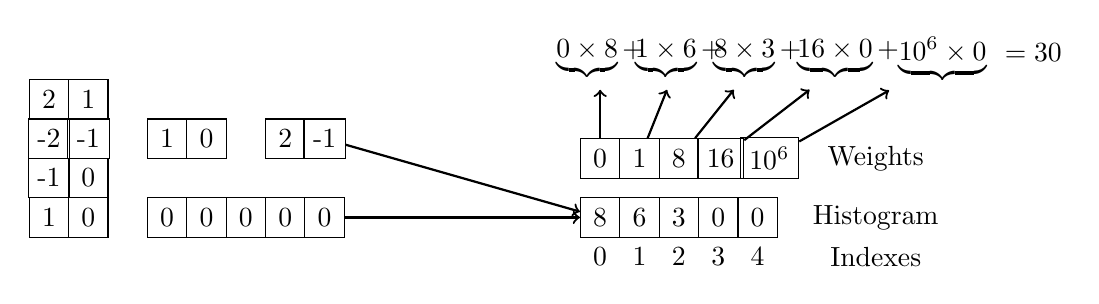
\begin{tikzpicture}

				\node [draw, minimum width=0.5cm, minimum height=0.5cm] at (0, 0) {1};
				\node [draw, minimum width=0.5cm, minimum height=0.5cm] at (0.5, 0) {0};
				\node [draw, minimum width=0.5cm, minimum height=0.5cm] at (0, 0.5) {-1};
				\node [draw, minimum width=0.5cm, minimum height=0.5cm] at (0.5, 0.5) {0};
				\node [draw, minimum width=0.5cm, minimum height=0.5cm] at (0, 1) {-2};
				\node [draw, minimum width=0.5cm, minimum height=0.5cm] at (0.5, 1) {-1};
				\node [draw, minimum width=0.5cm, minimum height=0.5cm] at (0, 1.5) {2};
				\node [draw, minimum width=0.5cm, minimum height=0.5cm] at (0.5, 1.5) {1};


				\node [draw, minimum width=0.5cm, minimum height=0.5cm] at (1.5, 0) {0};
				\node [draw, minimum width=0.5cm, minimum height=0.5cm] at (2.0, 0) {0};
				\node [draw, minimum width=0.5cm, minimum height=0.5cm] at (2.5, 0) {0};
				\node [draw, minimum width=0.5cm, minimum height=0.5cm] at (3.0, 0) {0};
				\node [draw, minimum width=0.5cm, minimum height=0.5cm] (C1) at (3.5, 0) {0};

				\node [draw, minimum width=0.5cm, minimum height=0.5cm] at (1.5, 1) {1};
				\node [draw, minimum width=0.5cm, minimum height=0.5cm] at (2.0, 1) {0};

				\node [draw, minimum width=0.5cm, minimum height=0.5cm] at (3.0, 1) {2};
				\node [draw, minimum width=0.5cm, minimum height=0.5cm] (C0) at (3.5, 1) {-1};


				\node [draw, minimum width=0.5cm, minimum height=0.5cm] (H0) at (7.0, 0) {8};
				\node [draw, minimum width=0.5cm, minimum height=0.5cm] at (7.5, 0) {6};
				\node [draw, minimum width=0.5cm, minimum height=0.5cm] at (8.0, 0) {3};
				\node [draw, minimum width=0.5cm, minimum height=0.5cm] at (8.5, 0) {0};
				\node [draw, minimum width=0.5cm, minimum height=0.5cm] at (9.0, 0) {0};

				\node [draw, minimum width=0.5cm, minimum height=0.5cm] (W0) at (7.0, 0.75) {0};
				\node [draw, minimum width=0.5cm, minimum height=0.5cm] (W1) at (7.5, 0.75) {1};
				\node [draw, minimum width=0.5cm, minimum height=0.5cm] (W2) at (8.0, 0.75) {8};
				\node [draw, minimum width=0.5cm, minimum height=0.5cm] (W3) at (8.53, 0.75) {16};
				\node [draw, minimum width=0.5cm, minimum height=0.5cm] (W4) at (9.15, 0.75) {$10^6$};
				\node at (10.5, 0.75) {Weights};
				\node at (10.5, 0) {Histogram};
				\node at (10.5, -0.5) {Indexes};

				\node at (7.0, -0.5) {0};
				\node at (7.5, -0.5) {1};
				\node at (8.0, -0.5) {2};
				\node at (8.5, -0.5) {3};
				\node at (9.0, -0.5) {4};

				\node (ID0) at (7.0, 2) {$\underbrace{0\times8} + $};
				\node (ID1) at (8.0, 2) {$\underbrace{1\times6} +$};
				\node (ID2) at (9.0, 2) {$\underbrace{8\times3} +$};
				\node (ID3) at (10.15, 2) {$\underbrace{16\times0} +$};
				\node (ID4) at (11.35, 2) {$\underbrace{10^6 \times 0}$};
				\node (ID5) at (12.5, 2.10) {$ = 30$};

				\draw [->,thick] (W0) -- (ID0);
				\draw [->,thick] (W1) -- (ID1);
				\draw [->,thick] (W2) -- (ID2);
				\draw [->,thick] (W3) -- (ID3);
				\draw [->,thick] (W4) -- (ID4);

				
				\draw [->,thick] (C0) -- (H0);
				\draw [->,thick] (C1) -- (H0);
		\end{tikzpicture}
		\caption{The four matrices obtained after applying the four masks on the matrix that represent the dot, in Figure~\ref{fig:dot-representation}.
						This Figure also represents the conversion to a histogram and how this histogram is used to find the heuristic value for the dot player.}
		\label{fig:convolution-results}
\end{figure}

\clearpage
\subsection{Vspace}
\label{sec:vspace}
The goal of the Vspace heuristic is to give value to empty
cells in addition to counting rows of similar
symbols. Similarly to the previous heuristic,
\textit{Vspace} counts the size of the lines, but for every
line connected to an empty cell, it uses the
size of this line as a value for the empty cell.

Figure~\ref{fig:dot-vspace} and
Figure~\ref{fig:color-vspace} give examples on
how the spaces are valued for both players, based
on the board at Figure~\ref{fig:board-example}.
Figure~\ref{fig:color-vspace} shows that even if
the line is split in two with an empty cell in the
middle, the combined value of both side gives the
value of the space. This is the reason why the two
3-values appears even though there is no line of
three.

Possible value for spaces range from 0 to 4 and
higher values are downed to 4. When multiple lines
are connected to an empty cell, the cell receives
the maximum value from them. The heuristic split the
space into two categories: the space available in
the next turn and the spaces too high to be
reached with one card.

Finally, a histogram for each category is made and
each value is multiplied by a weight then summed.
Note that the two categories have different
weights because a space connected to a line of
three symbols does not hold the same value if you
can play on it on the next turn or not.
\begin{figure}[ht]
		\center
		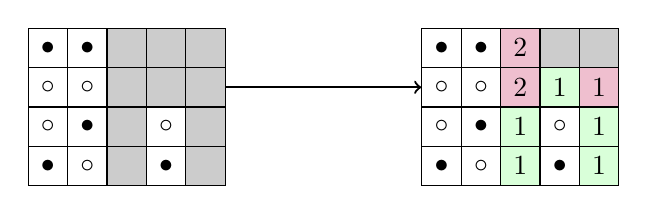
\begin{tikzpicture}

				\node [draw, minimum width=0.5cm, minimum height=0.5cm] at (0, 0) {$\bullet$};
				\node [draw, minimum width=0.5cm, minimum height=0.5cm] at (0.5, 0) {$\circ$};
				\node [draw, fill=black!20, minimum width=0.5cm, minimum height=0.5cm] at (1.0, 0) {};
				\node [draw, minimum width=0.5cm, minimum height=0.5cm] at (1.5, 0) {$\bullet$};
				\node [draw, fill=black!20, minimum width=0.5cm, minimum height=0.5cm] at (2.0, 0) {};


				\node [draw, minimum width=0.5cm, minimum height=0.5cm] at (0, 0.5) {$\circ$};
				\node [draw, minimum width=0.5cm, minimum height=0.5cm] at (0.5, 0.5) {$\bullet$};
				\node [draw, fill=black!20, minimum width=0.5cm, minimum height=0.5cm] at (1.0, 0.5) {};
				\node [draw, minimum width=0.5cm, minimum height=0.5cm] at (1.5, 0.5) {$\circ$};
				\node [draw, fill=black!20, minimum width=0.5cm, minimum height=0.5cm] at (2.0, 0.5) {};


				\node [draw, minimum width=0.5cm, minimum height=0.5cm] at (0, 1) {$\circ$};
				\node [draw, minimum width=0.5cm, minimum height=0.5cm] at (0.5, 1) {$\circ$};
				\node [draw, fill=black!20, minimum width=0.5cm, minimum height=0.5cm] at (1.0, 1) {};
				\node [draw, fill=black!20, minimum width=0.5cm, minimum height=0.5cm] at (1.5, 1) {};
				\node [draw, fill=black!20, minimum width=0.5cm, minimum height=0.5cm] (A) at (2.0, 1) {};

				\node [draw, minimum width=0.5cm, minimum height=0.5cm] at (0, 1.5) {$\bullet$};
				\node [draw, minimum width=0.5cm, minimum height=0.5cm] at (0.5, 1.5) {$\bullet$};
				\node [draw, fill=black!20, minimum width=0.5cm, minimum height=0.5cm] at (1.0, 1.5) {};
				\node [draw, fill=black!20, minimum width=0.5cm, minimum height=0.5cm] at (1.5, 1.5) {};
				\node [draw, fill=black!20, minimum width=0.5cm, minimum height=0.5cm] at (2.0, 1.5) {};

				%------
				\node [draw, minimum width=0.5cm, minimum height=0.5cm] at (5, 0) {$\bullet$};
				\node [draw, minimum width=0.5cm, minimum height=0.5cm] at (5.5, 0) {$\circ$};
				\node [draw, fill=green!15, minimum width=0.5cm, minimum height=0.5cm] at (6.0, 0) {1};
				\node [draw, minimum width=0.5cm, minimum height=0.5cm] at (6.5, 0) {$\bullet$};
				\node [draw, fill=green!15, minimum width=0.5cm, minimum height=0.5cm] at (7.0, 0) {1};


				\node [draw, minimum width=0.5cm, minimum height=0.5cm] at (5, 0.5) {$\circ$};
				\node [draw, minimum width=0.5cm, minimum height=0.5cm] at (5.5, 0.5) {$\bullet$};
				\node [draw, fill=green!15, minimum width=0.5cm, minimum height=0.5cm] at (6.0, 0.5) {1};
				\node [draw, minimum width=0.5cm, minimum height=0.5cm] at (6.5, 0.5) {$\circ$};
				\node [draw, fill=green!15, minimum width=0.5cm, minimum height=0.5cm] at (7.0, 0.5) {1};


				\node [draw, minimum width=0.5cm, minimum height=0.5cm] (B) at (5, 1) {$\circ$};
				\node [draw, minimum width=0.5cm, minimum height=0.5cm] at (5.5, 1) {$\circ$};
				\node [draw, fill=purple!25, minimum width=0.5cm, minimum height=0.5cm] at (6.0, 1) {2};
				\node [draw, fill=green!15, minimum width=0.5cm, minimum height=0.5cm] at (6.5, 1) {1};
				\node [draw, fill=purple!25, minimum width=0.5cm, minimum height=0.5cm] at (7.0, 1) {1};

				\node [draw, minimum width=0.5cm, minimum height=0.5cm] at (5, 1.5) {$\bullet$};
				\node [draw, minimum width=0.5cm, minimum height=0.5cm] at (5.5, 1.5) {$\bullet$};
				\node [draw, fill=purple!25, minimum width=0.5cm, minimum height=0.5cm] at (6.0, 1.5) {2};
				\node [draw, fill=black!20, minimum width=0.5cm, minimum height=0.5cm] at (6.5, 1.5) {};
				\node [draw, fill=black!20, minimum width=0.5cm, minimum height=0.5cm] at (7.0, 1.5) {};

				\draw [->,thick] (A) -- (B);
		\end{tikzpicture}
		\caption{Example of the Vspace process for the
		dot player based on the board in
		Figure~\ref{fig:board-example}. the grey cells
		represent cells that contain nothing
		interesting. On the right board, green cells
		are spaces available for the next turn and
		purple cells are spaces that need at least two
		cards to be filled.}
		\label{fig:dot-vspace}
\end{figure}
\begin{figure}[ht]
		\center
		\begin{tikzpicture}

				\node [draw, fill=red!20, minimum width=0.5cm, minimum height=0.5cm] at (0, 0) {};
				\node [draw, fill=red!20, minimum width=0.5cm, minimum height=0.5cm] at (0.5, 0) {};
				\node [draw, fill=black!20, minimum width=0.5cm, minimum height=0.5cm] at (1.0, 0) {};
				\node [draw, fill=red!20, minimum width=0.5cm, minimum height=0.5cm] at (1.5, 0) {};
				\node [draw, fill=black!20, minimum width=0.5cm, minimum height=0.5cm] at (2.0, 0) {};


				\node [draw, minimum width=0.5cm, minimum height=0.5cm] at (0, 0.5) {};
				\node [draw, minimum width=0.5cm, minimum height=0.5cm] at (0.5, 0.5) {};
				\node [draw, fill=black!20, minimum width=0.5cm, minimum height=0.5cm] at (1.0, 0.5) {};
				\node [draw, minimum width=0.5cm, minimum height=0.5cm] at (1.5, 0.5) {};
				\node [draw, fill=black!20, minimum width=0.5cm, minimum height=0.5cm] at (2.0, 0.5) {};


				\node [draw, fill=red!20, minimum width=0.5cm, minimum height=0.5cm] at (0, 1) {};
				\node [draw, minimum width=0.5cm, minimum height=0.5cm] at (0.5, 1) {};
				\node [draw, fill=black!20, minimum width=0.5cm, minimum height=0.5cm] at (1.0, 1) {};
				\node [draw, fill=black!20, minimum width=0.5cm, minimum height=0.5cm] at (1.5, 1) {};
				\node [draw, fill=black!20, minimum width=0.5cm, minimum height=0.5cm] at (2.0, 1) {};

				\node [draw, minimum width=0.5cm, minimum height=0.5cm] at (0, 1.5) {};
				\node [draw, fill=red!20, minimum width=0.5cm, minimum height=0.5cm] at (0.5, 1.5) {};
				\node [draw, fill=black!20, minimum width=0.5cm, minimum height=0.5cm] at (1.0, 1.5) {};
				\node [draw, fill=black!20, minimum width=0.5cm, minimum height=0.5cm] at (1.5, 1.5) {};
				\node [draw, fill=black!20, minimum width=0.5cm, minimum height=0.5cm] at (2.0, 1.5) {};

				%------
				\node [draw, fill=red!20, minimum width=0.5cm, minimum height=0.5cm] at (5, 0) {};
				\node [draw, fill=red!20, minimum width=0.5cm, minimum height=0.5cm] at (5.5, 0) {};
				\node [draw, fill=green!15, minimum width=0.5cm, minimum height=0.5cm] at (6.0, 0) {3};
				\node [draw, fill=red!20, minimum width=0.5cm, minimum height=0.5cm] at (6.5, 0) {};
				\node [draw, fill=green!15, minimum width=0.5cm, minimum height=0.5cm] at (7.0, 0) {1};


				\node [draw, minimum width=0.5cm, minimum height=0.5cm] at (5, 0.5) {};
				\node [draw, minimum width=0.5cm, minimum height=0.5cm] at (5.5, 0.5) {};
				\node [draw, fill=green!15, minimum width=0.5cm, minimum height=0.5cm] at (6.0, 0.5) {3};
				\node [draw, minimum width=0.5cm, minimum height=0.5cm] at (6.5, 0.5) {};
				\node [draw, fill=green!15, minimum width=0.5cm, minimum height=0.5cm] at (7.0, 0.5) {1};


				\node [draw, fill=red!20, minimum width=0.5cm, minimum height=0.5cm] (B) at (5, 1) {};
				\node [draw, minimum width=0.5cm, minimum height=0.5cm] at (5.5, 1) {};
				\node [draw, fill=purple!25, minimum width=0.5cm, minimum height=0.5cm] at (6.0, 1) {1};
				\node [draw, fill=green!15, minimum width=0.5cm, minimum height=0.5cm] at (6.5, 1) {1};
				\node [draw, fill=purple!25, minimum width=0.5cm, minimum height=0.5cm] at (7.0, 1) {1};

				\node [draw, minimum width=0.5cm, minimum height=0.5cm] at (5, 1.5) {};
				\node [draw, fill=red!20, minimum width=0.5cm, minimum height=0.5cm] at (5.5, 1.5) {$\bullet$};
				\node [draw, fill=purple!25, minimum width=0.5cm, minimum height=0.5cm] at (6.0, 1.5) {2};
				\node [draw, fill=black!20, minimum width=0.5cm, minimum height=0.5cm] at (6.5, 1.5) {};
				\node [draw, fill=black!20, minimum width=0.5cm, minimum height=0.5cm] at (7.0, 1.5) {};

				\draw [->,thick] (A) -- (B);
		\end{tikzpicture}
		\caption{Example of the Vspace process for the
		color player based on the board in
		Figure~\ref{fig:board-example}. the grey cells
		represent cells that contain nothing
		interesting. On the right board, green cells
		are spaces available for the next turn and
		purple cells are spaces that need at least two
		cards to be filled.}
		\label{fig:color-vspace}
\end{figure}

The default weights of \textit{Vspace} were hinted
by a genetic algorithm~\cite{genetic}. The DEAP~\cite{deap}
library was used to improve the initial weights
which were a simple guess.  New weights would
compete against a \textit{Vspace} heuristic with
the original weights and the winning rate was used
to evaluate them. In case the winning rate was
zero, the new canditates were sorted by the
average length of their game: the longer, the
better. After a night of simulation, the results
indicate that lines should not be counted except
for lines of four symbols.  This change,
greatly improved the winning rate of
\textit{Vspace}.

\clearpage
\section{Difficulties}
The biggest difficulty encountered during this
project was the slowness of python. In the early
stage of the project, the code was
too inefficient and could not check more than one
move in advance within the limit of three seconds. 

\textit{cProfile}~\cite{cprofile} is a module to profile
python code. In particular,
it gives the amount of time spent in each function
called. This profiler was used to locate the most
time-consuming function, then this information
helps to restructure the code and enhance the
performance.

However, the results were hardly perceivable and
the code remains slow even with the later use of
optimized python libraries (Numpy and Scipy
\cite{numpy}). Functions from these libraries rely
on built-in functions which are written in C, then
compiled into python module.  Therefore, the use
of this type of function should improve the speed
of the engine.

However, none of the approaches above provide significant improvement. Finally,
to reach a decent executing time for the tournament, one last step was taken
and a python module written in C was developed.
Figure~\ref{fig:performance-magic} shows the
evolution of the performances as the most time-consuming function given by \textit{cProfile} were adapted to call the
module. However, the python code remains and it is
executed by default. 
Figure~\ref{fig:performance-magic} shows that the
MinMax algorithm is able to check four moves in
advance after half of the key part used the
module.

\begin{figure}
		\centering
		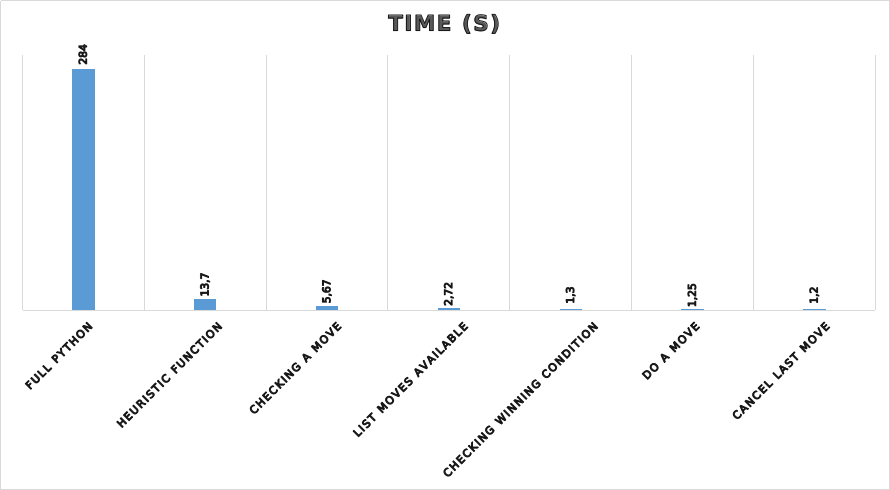
\includegraphics[width=0.8\textwidth]{perfromances.png}
		\caption{The amount of time (in seconds) taken
		to run the MinMax algorithm on a board with the
		card "5 B 1" already played. The MinMax
		algorithm checked up to four moves in advance and
		it used the Vspace heuristic described in
		Section~\ref{sec:vspace}. The left column
		shows the full python execution time (more
		than 4 minutes) and the other columns show the
		execution time as part of the code start using
		the C module. The third column from the left,
		"checking a move", indicate the time taken
		when the heuristic function and the function
		that check the moves use both the C module.}
		\label{fig:performance-magic}
\end{figure}

\clearpage
\section{Analyze}
This section presents three analyses. A comparison
between the two heuristics; a brief  overview of
the alpha-beta pruning impact; and an experiment
where the branching factor is limited in order to
go deeper.

Before exploring these analyses, a brief
explanation about winning rate tables. When two
heuristics/algorithms are compared, two situations
are considered: one algorithm
play first in the first situation then the roles
are inverted in the next situation. A quick experiment with the
same algorithm and the same heuristic showed that
the winning rate is higher for the second player.
Therefore, we need to compare two situations.

\subsection{Heuristic comparison}
In this section, we compare the efficiency between
the two heuristics. Table~\ref{tab:win-heuristic}
shows the winning rate of each heuristic out of 20
games. \textit{Vspace} is used with a depth of
four (four moves in advance) while the convolution
only uses a depth of three. This difference in
depth appears because the \textit{Vspace}
heuristic is more optimized. Both heuristics are
used by the tweaked \textit{MinMax} algorithm described
above.

The first row of Table~\ref{tab:win-heuristic}
indicates that the \textit{Vspace} heuristic wins
70 \%  of the game when it starts to play while the
convolution heuristic wins the other 30 \%.
From this table, we see that the Vspace heuristic
performs better because it also wins all games
when the convolution heuristic plays first.

To investigate the efficiency of the heuristic
rather than the combination of its performance and
efficiency, the previous experiment was redone
with both heuristics using the same depth.
Table~\ref{tab:win-heuristic-same} shows the
winning ratio for this second experiment. We
denote that the \textit{Vspace} heuristic is more
efficient than the convolution. 

\begin{table}
	\begin{subtable}{0.5\textwidth}
		\centering
		\caption{Optimal depth}\label{tab:win-heuristic}
		\begin{tabular}{|l|l|l|}
		\hline
		First player &  Vspace & Convolution\\
		\hline
		 Vspace 		 &  70 \% & 30 \%\\
		 Convolution &  100 \% & 0 \%\\
		\hline
		\end{tabular}
	\end{subtable}
	\begin{subtable}{0.49\textwidth}
		\centering
		\caption{Same depth}\label{tab:win-heuristic-same}
		\begin{tabular}{|l|l|l|}
		\hline
		First player &  Vspace & Convolution\\
		\hline
		 Vspace 		 &  55 \% & 45 \%\\
		 Convolution &  100 \% & 0 \%\\
		\hline
		\end{tabular}
	\end{subtable}
	\caption{Shows the winning ratio between the two
		heuristics. On the left, both heuristics use
		the maximum depth they could reach. On the
		right, they use the same depth (three moves
		in advance). The column \textit{First player}
		indicates which heuristic is playing first.}
\end{table}

\subsection{Alpha-Beta}
The impact of Alpha-Beta pruning is important. A
quick experiment with the \textit{Vspace}
heuristic on depth 4 showed that the alpha-beta
pruning speed-up the algorithm by a factor of 26
(from 43 seconds to 1.6 seconds). The efficiency
of the pruning is also seen in the number of time the
heuristic function is called: 90000 calls with the
pruning and more than 4 million without.
Therefore, we can conclude that the Alpha-Beta
pruning is a key element of the \textit{MinMax}.

\subsection{Limiting the width}
During the tournament, I heard that a team added a
limitation in width in addition to the depth
limitation.
Therefore, I decided to evaluate this idea in my
own project. I design a new version of the MinMax
algorithm where at the beginning of each function
(\textit{min} and \textit{max}) each move is rated
with the heuristic and only the 25 best are
explored. This modification fixed the branching
factor at 25 and allows the algorithm to go
one level deeper. The factor of 25 was choosen
because it allows going just one level deeper
within the time limit while still exploring many
moves.

Table~\ref{tab:win-limit-width} shows the win rate
between the \textit{MinMax} with unlimited width
and the one with a branching factor of 25. The Table
reveals that the limited search with one level
deeper has a poor winning rate whether it starts
to play or not.
Therefore, in this project with the
\textit{Vspace} heuristic, limiting the width is inefficient
and does not give an advantage.
\begin{table}
		\centering
		\caption{Win ratio when the width is limited.}\label{tab:win-limit-width}
		\begin{tabular}{|l|l|l|}
		\hline
		First player &  Limited & Unlimited\\
		\hline
		 Limited &  0 \% & 100 \%\\
		 Unlimited &  35 \% & 65 \%\\
		\hline
		\end{tabular}
\end{table}


\section{Conclusion}
This project taught me many things about AI
programming for two player game. It showed me how
the weight of a heuristic can be optimized. It
proved me that going deeper in the state tree
is not the better option if all possibilities are
not properly explored. Finally, I learned to program python
module and to combine the performance of C with
the simplicity of python when performances are
required.
\bibliographystyle{splncs04}
\bibliography{paper}
\end{document}

% vim: tw=50 ts=2
